\documentclass[UFT8]{article}
\usepackage{ctex}%中文
\usepackage{amsmath}
\usepackage{graphicx}%插图
\usepackage[bookmarks=true,colorlinks,linkcolor=black]{hyperref}%书签和链接
\usepackage{amstext}%数学环境中的文字
\usepackage{esint}%曲面积分符号
\usepackage{pgfplots}%画函数图像
\usepackage{eucal}%特殊数学字体
\usepackage{geometry}
\geometry{a4paper,scale=0.8}
\begin{document}
\kaishu
\title{光学笔记}
\author{zhufeng}
\date{}
\maketitle
\thispagestyle{empty}
\newpage
\tableofcontents
\newpage
\pagenumbering{arabic}%从正文开始计算页码
\thispagestyle{empty}
\setcounter{page}{1}
\section{干涉}
\subsection{杨氏双缝干涉实验}
\textbf{相干性}:通常频率相同,振动在一条直线上。相位差恒定的两个振动是相干的,注意此时的振动方向是不一定一致的,干涉光强公式给出:\\
干涉相长:
\[
	I=I_1+I_2+2\sqrt{I_1I_2}
\]
干涉相消:
\[
	I=I_1+I_2-2\sqrt{I_1I_2}
\]
这里给出杨氏双缝干涉的原理图:
\begin{figure*}[htpb]
\begin{center}
\raisebox{-0.5\height}{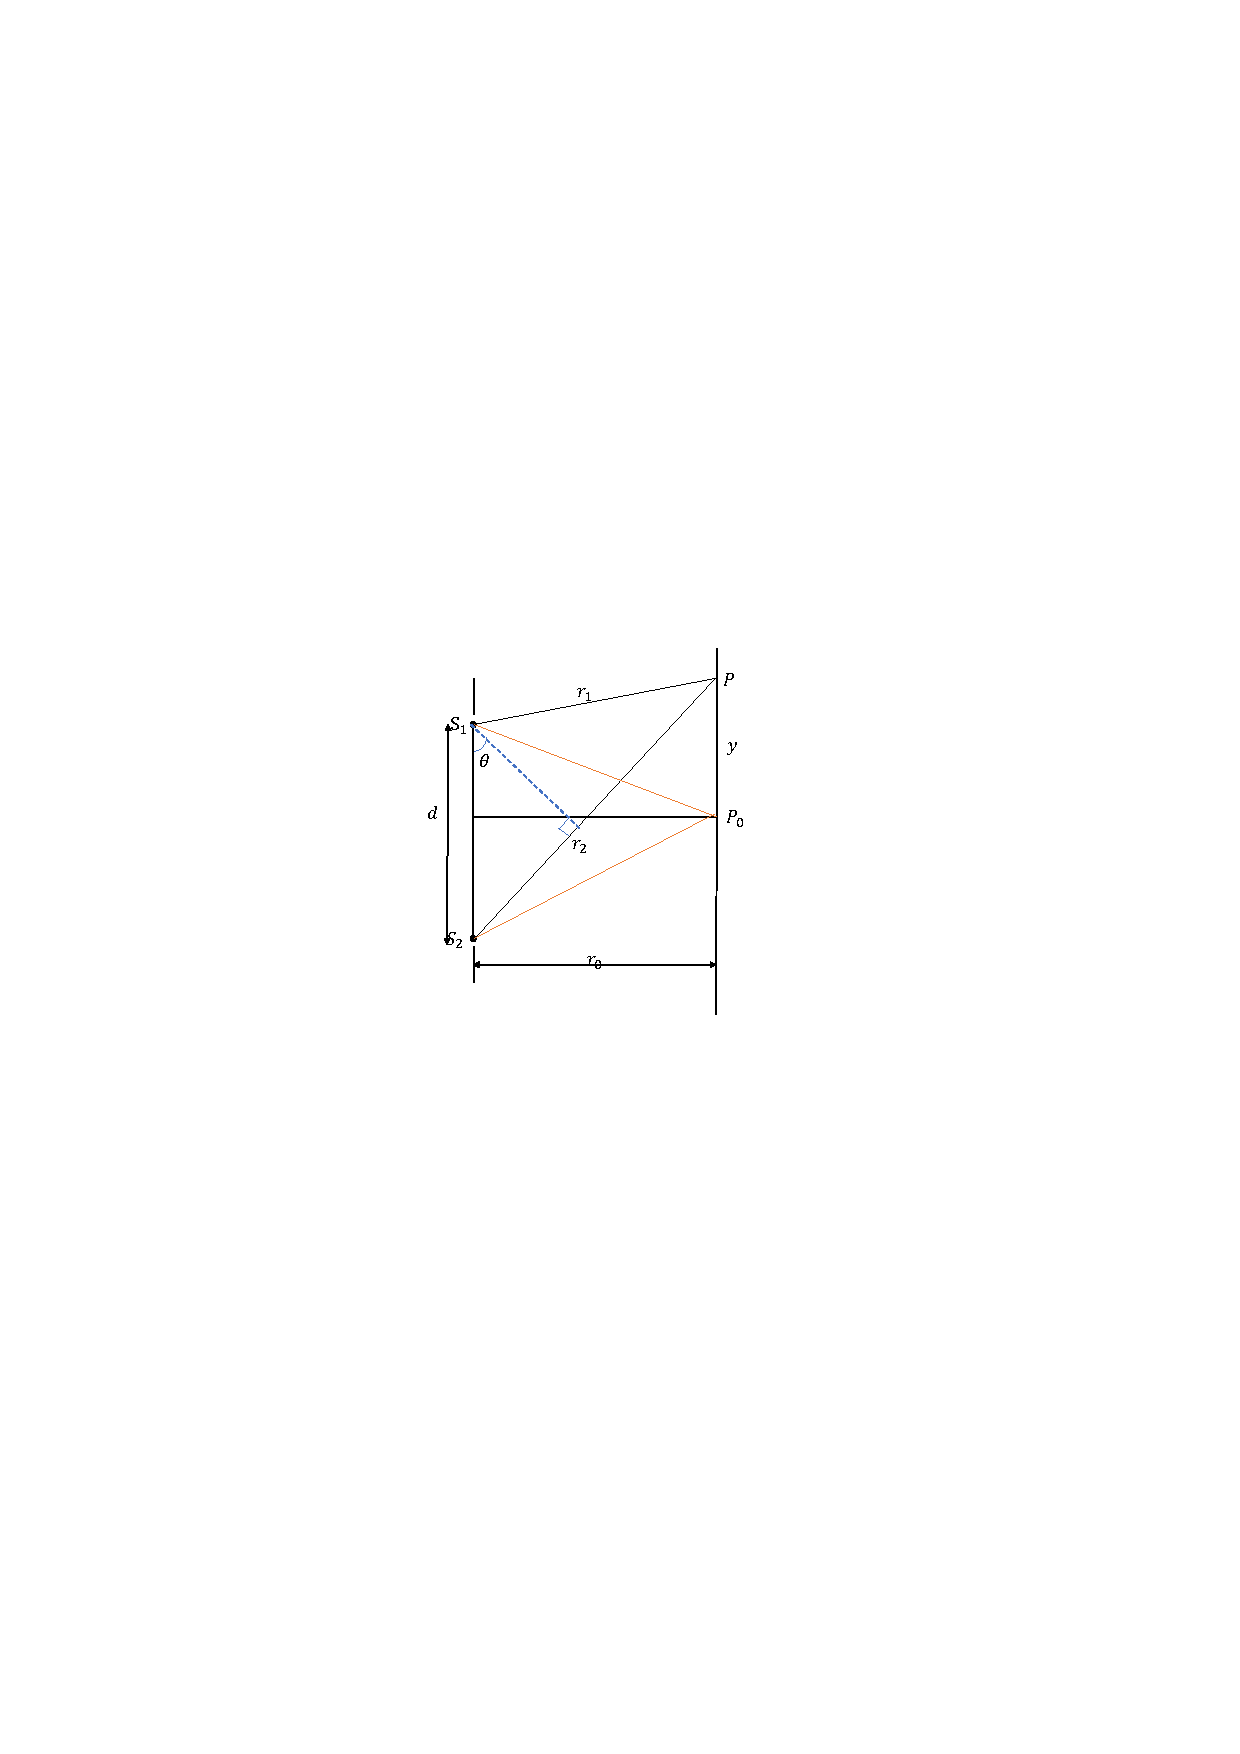
\includegraphics[width=7.8909550045914cm,height=6.92450478814115cm]{干涉.pdf}}
\end{center}
\caption{杨氏双缝干涉的原理图}
\end{figure*}

因此由单色波形成的干涉条纹:
\begin{equation*}
r_2-r_1=
\begin{cases}
(2j)\frac{\lambda}{2}\\
(2j+1)\frac{\lambda}{2}
\end{cases}
\end{equation*}

我们继续可以由几何关系得到:
\begin{align*}
d\sin \theta=d\frac{y}{r_0}\\
d\frac{\Delta y}{r_0}=\lambda\Rightarrow\Delta y=\frac{r_0\lambda}{d}
\end{align*}
分波面双光束干涉
\begin{figure*}[htpb]
\begin{center}
\raisebox{-0.5\height}{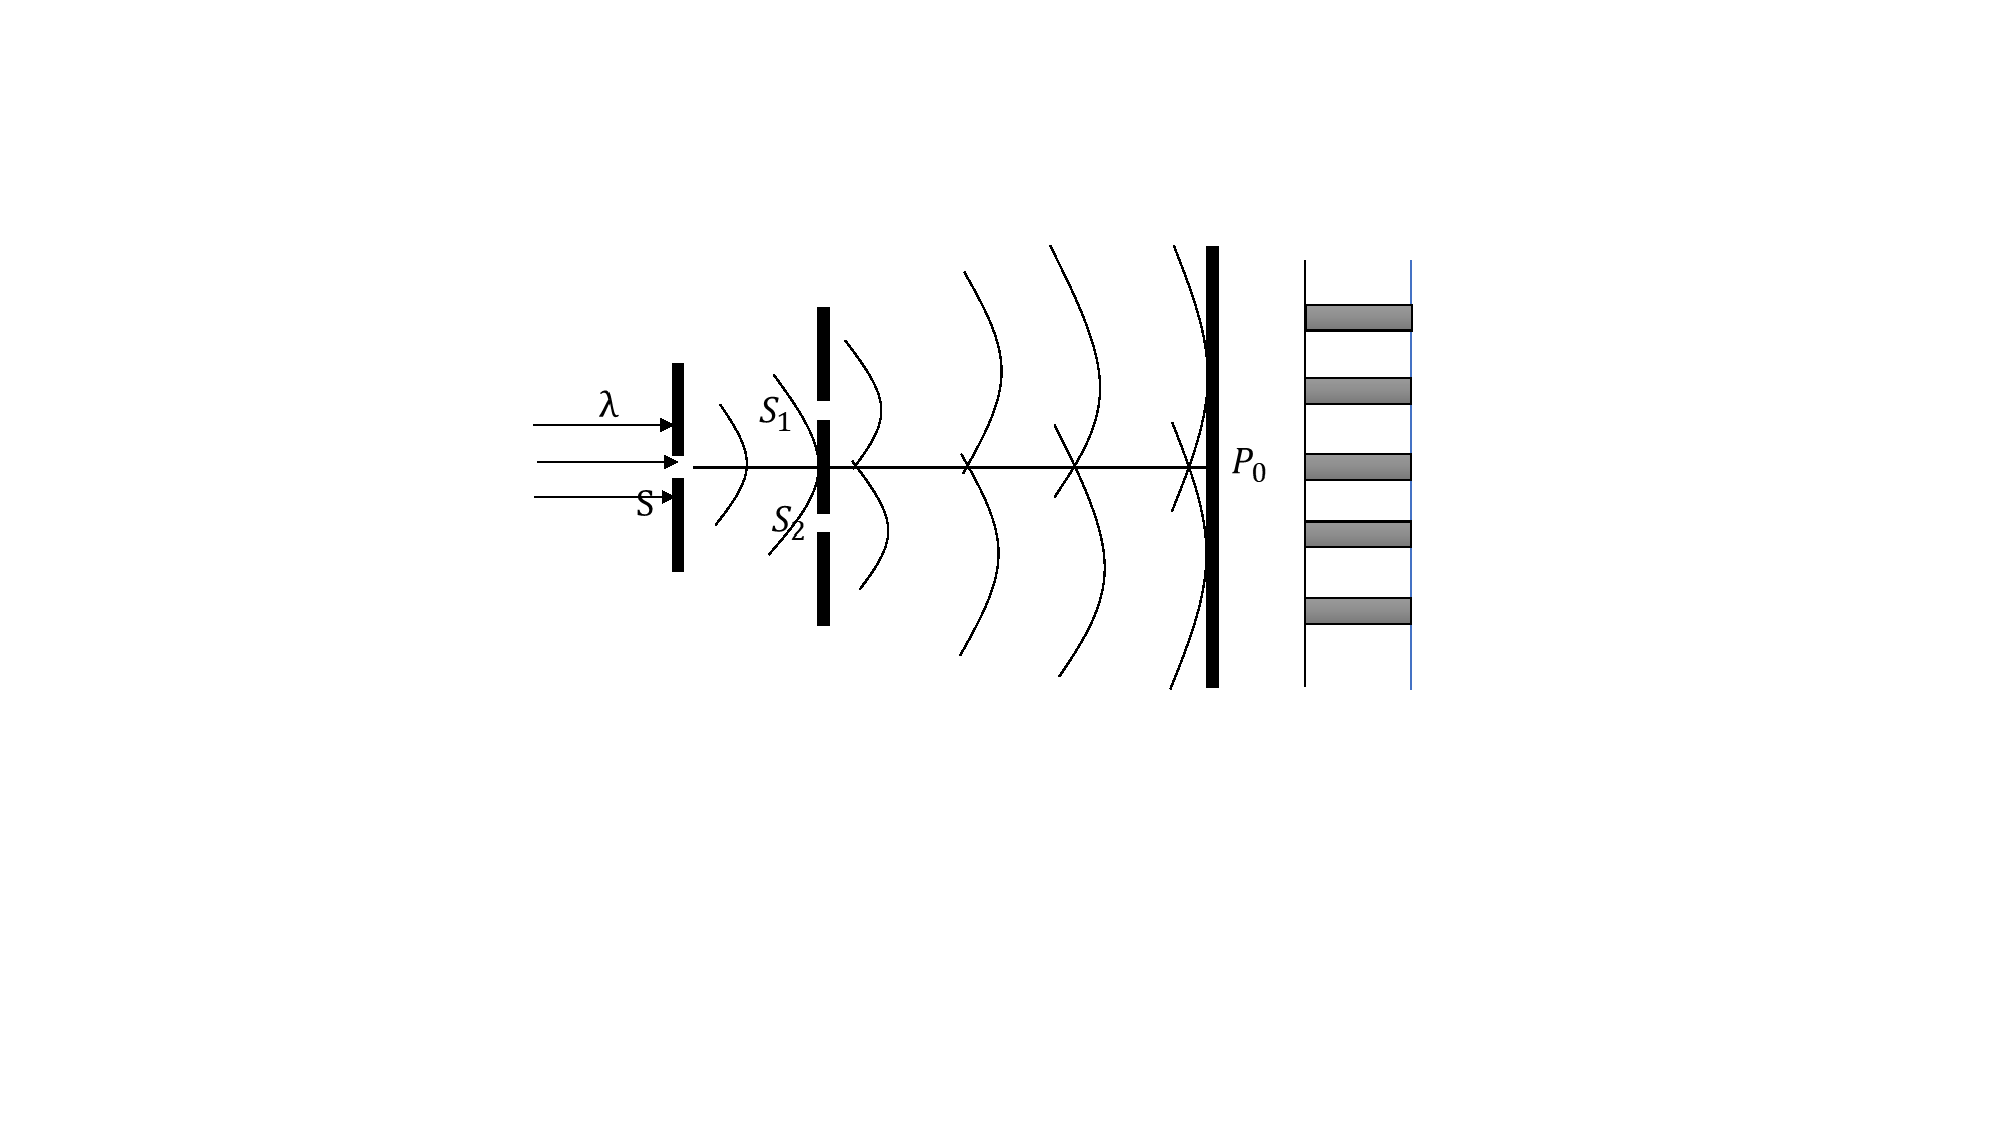
\includegraphics[width=6cm,height=3cm]{波形.pdf}}
\end{center}
\caption{分波面双光束干涉}
\end{figure*}

\subsection{光源的极限宽度-线度}
\begin{figure*}[htpb]
\begin{center}
\raisebox{-0.5\height}{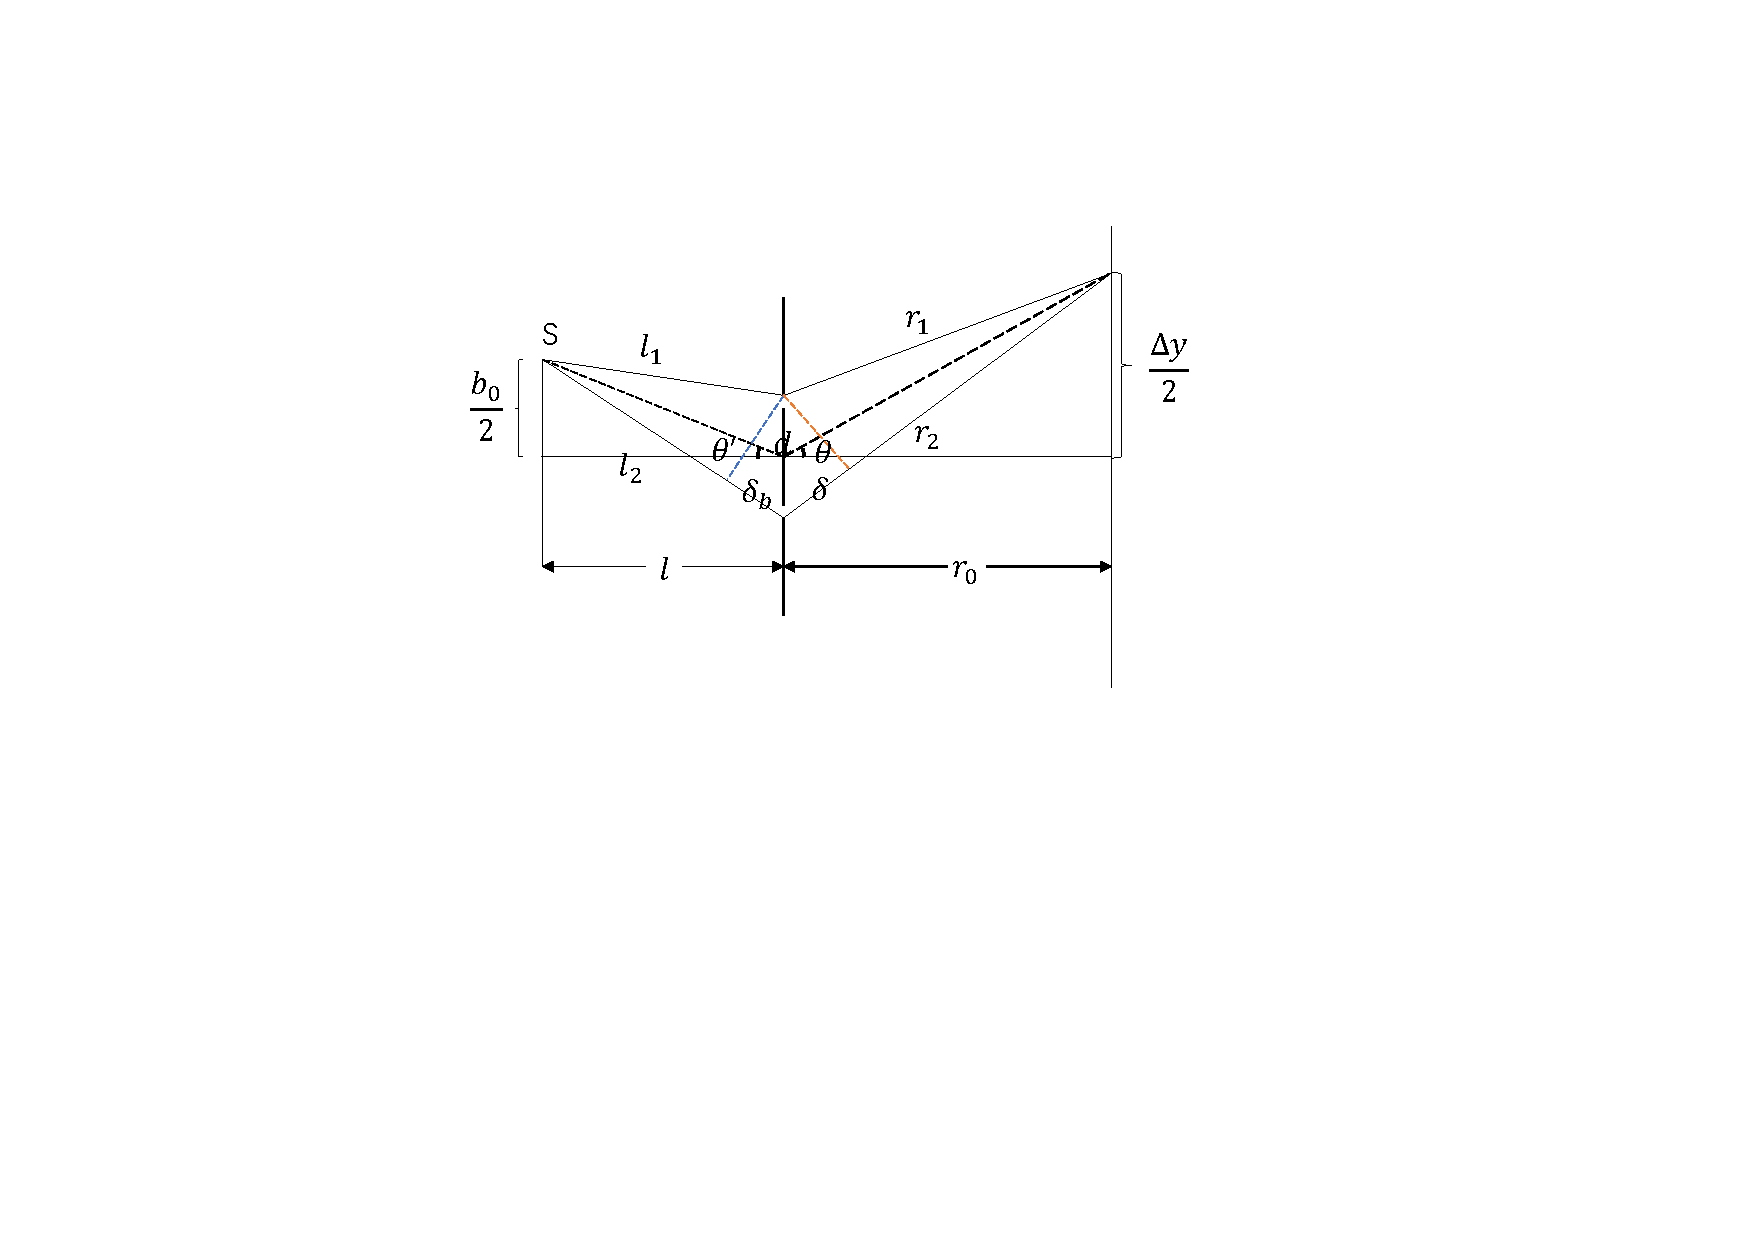
\includegraphics[width=6cm,height=4cm]{线度.pdf}}
\end{center}
\caption{线度原理图}
\end{figure*}

光源上的端点:
\[
	(r_2+l_2)(r_1+l_1)=\delta+\delta_b=\lambda
\]
光源中点:
\[
	\delta=d\sin \theta=d\frac{\Delta y/2}{r_0}=\frac{\lambda}{2}
\]
最终我们得到:
\[
	\delta_b\approx d\sin\theta'=d\frac{b_0/2}{l}
\]
\subsection{半波损失}
条件,光线从光疏介质到光密介质时,反射光发生半个波长的损失(注意入射角要很小),在劳埃德镜中的半波损失现象,由于发生了半个波长的损失,在原本应该出现亮纹的地方出现了暗纹,在原本出现暗纹的地方出现了亮纹,因为以后的波长都损失了半个波长。
\subsection{等倾干涉}
\begin{figure*}[htbp]
\begin{center}
\raisebox{-0.5\height}{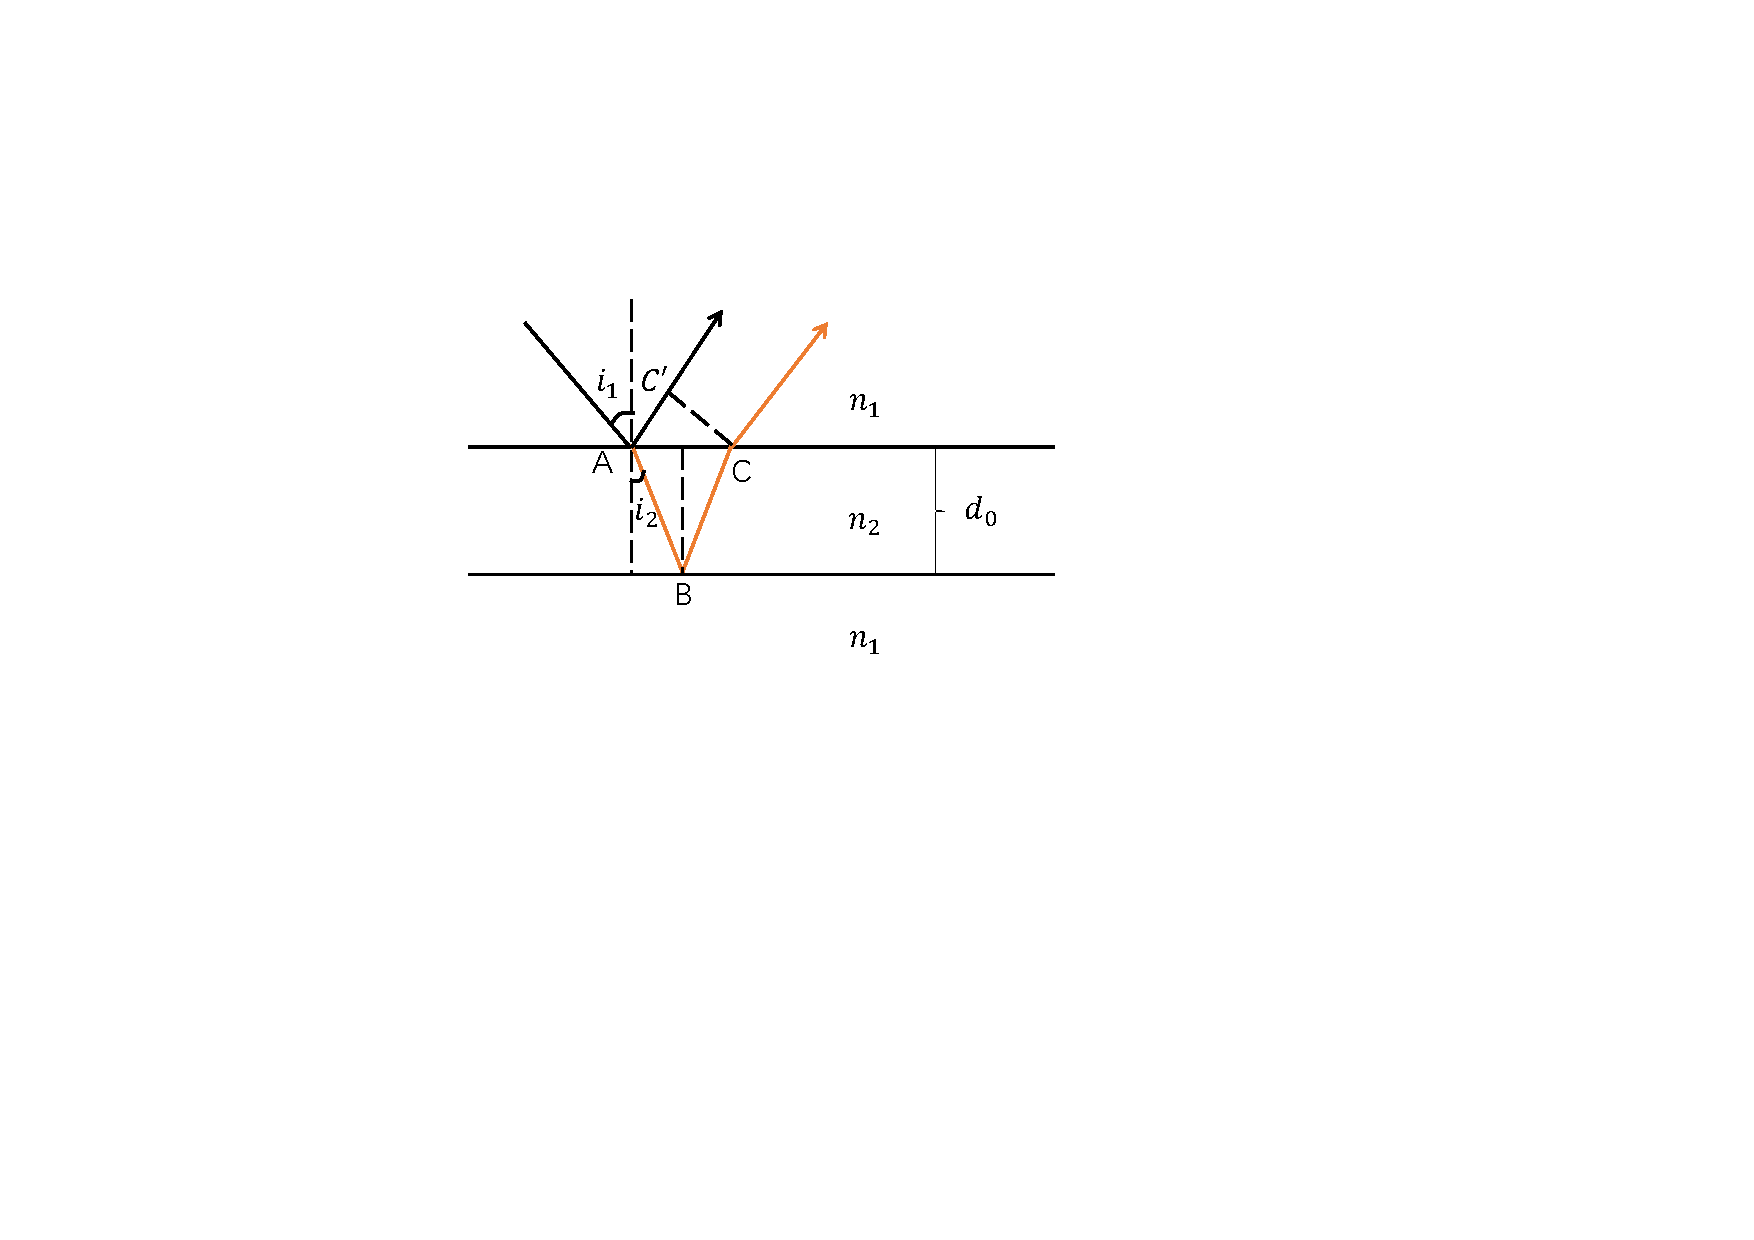
\includegraphics[width=7cm,height=4cm]{等倾干涉.pdf}}
\end{center}
\caption{等倾干涉示意图}
\end{figure*}

注意等倾干涉倾角不同:光程差分析:$\delta=AB+BC-AC'$然后利用几何关系得出光程差公式,\textbf{注意从光疏介质到光密介质会发生半波损失},
\begin{align*}
\sigma=2d_0\sqrt{n_{2}^{2}-n_{1}^{2}\sin^2 i_1}-\frac{\lambda}{2}=
\begin{cases}
(2j)\frac{\lambda}{2}\\
(2j+1)\frac{\lambda}{2}
\end{cases}
\end{align*}
现在对干涉条纹来分析可以得到分析其中一个亮纹就是可以的:
\begin{gather*}
2d_0n_2\cos i_1=(2j)\frac{\lambda}{2}\\
\cos i_2=(2j)\frac{\lambda}{4n_2 d_0}
\end{gather*}
在等倾干涉中i的大小是可以反应条纹的间距的:
\begin{gather*}
\sin i_2-\cos i_2'=\frac{\lambda}{2n_2d_0}\\
\cos x=\sum_{k=0}^{\infty}\frac{(-1)^k}{(2k)!}x^{2k}\\
i_{2}^{2}-i_{2}'^{2}=\frac{\lambda}{n_2 d_0}
\end{gather*}
对于垂直入射的等倾干涉来说,垂直入射由于d和i是相同的,所以所有位置处的光是同一种状态,所以得到的干涉图时:单色光入射时,根据d的不同时全部亮或者全部暗。
\subsection{等厚干涉}
\begin{figure*}[htbp]
\begin{center}
\raisebox{-0.5\height}{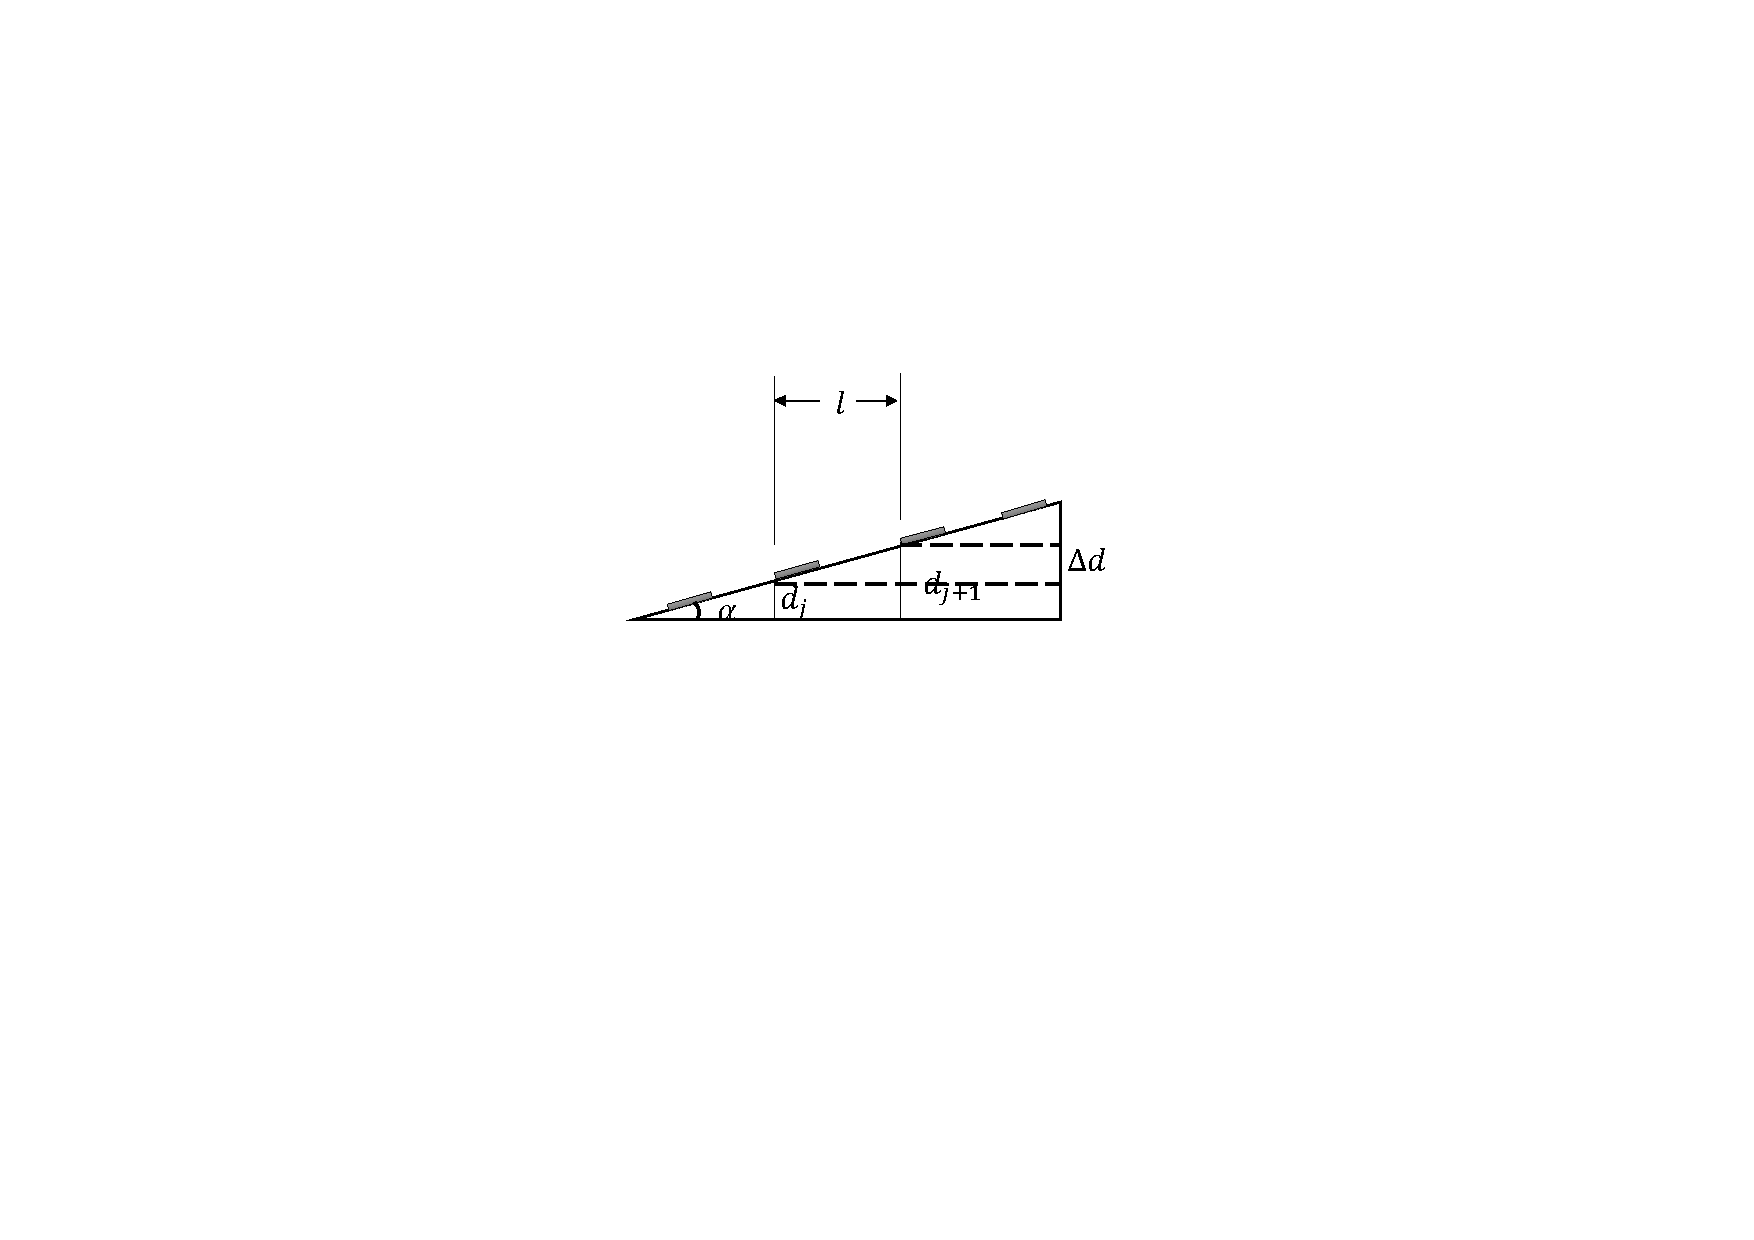
\includegraphics[width=6cm,height=4.5cm]{等厚干涉.pdf}}
\end{center}
\caption{等厚干涉示意图}
\end{figure*}
公式是和等倾干涉是一样的,但是,具体情况还是要具体分析:
此时分析垂直入射的光线:
\begin{gather*}
n_2\Delta d=\frac{\lambda}{2}\\
l=\frac{\Delta d}{\sin \alpha}
\end{gather*}
解方程得到:
\[
	l=\frac{\lambda}{2n_2\alpha}
\]

问题:当膜的厚度增加时,条纹移动的方向是怎么样的?\\
此时可以结合图像分析,当d增大时,左边的d就相当于右边的d,原本对应的右边的条纹现在对应到左边去了,所以此时的条纹应该是向左平移,当然这个也是可以用相关的公式来推导的
\[
	2d_0\sqrt{n_{2}^{2}-n_{1}^{2}\sin^2 i_1}=(2j)\frac{\lambda  }{2}
\]
d增大时,条纹的极次升高,极次高的到左边来了,可以理解为向左平移,图中的示意图都只是平面图像。\textbf{对于等厚干涉来说,高的地方极次高,低的地方极次低,干涉图样时等间距直线状}
\subsection{薄膜色}
用白光照射,可以看到彩色条纹。彩色条纹是由于不同的干涉级的某些波长发生干涉相消,某些波长发生干涉相长,相互叠加在一起后所形成的,所以这种彩色时混合色,不是单色,这种彩色通常称为薄膜色
\subsection{可见度}
条纹的可见度:
\[
	V=\frac{I_{max}-I_{min}}{I_{max}+I_{min}}
\]
当$I_{min}=0$时,可见度最大,条纹最清晰。\\
时间相干性:当一束光入射时,由于运动的距离是不一样的,会产生一点点的时间之差,当时间之差极小时,可以发生干涉现象,但是当时间大于某个特定值之后,两束光不能发生叠加\\
空间相干性:一般我们是把光源看成点光源,但是事实上,是存在一定的大小的,还需要指出的是,实际的实验中没有那么理想的点光源,因为线光源会在屏幕上发生叠加,导致恰好抵消之后可见度为0
\subsection{对点光源单色性的分析}
\begin{equation*}
d\sin \theta=
\begin{cases}
(2j)\frac{\lambda}{2}\\
(2j+1)\frac{\lambda}{2}
\end{cases}
\end{equation*}
就拿其中的一种情况来分析其单色性,此时:
\[
	d\sin\theta=(2j+1)\frac{\lambda}{2}=(2j)=\frac{\lambda+\Delta\lambda}{2}
\]
此时当波长$\lambda+\Delta\lambda$的第j级和$\lambda$的第j+1级重合时,干涉条纹会发生重叠,影响观察。所以对光源的单色性需要满足一定的条件
\section{光的衍射}
\subsection{惠更斯菲涅尔原理}
惠更斯只提出了光在遇到障碍物时,会在障碍物上形成一下新的次波,次波又是新的子波波源,只是指出了这么一个现象,而没有描述振幅和相位。
\begin{figure*}[htbp]
\begin{center}
\raisebox{-0.5\height}{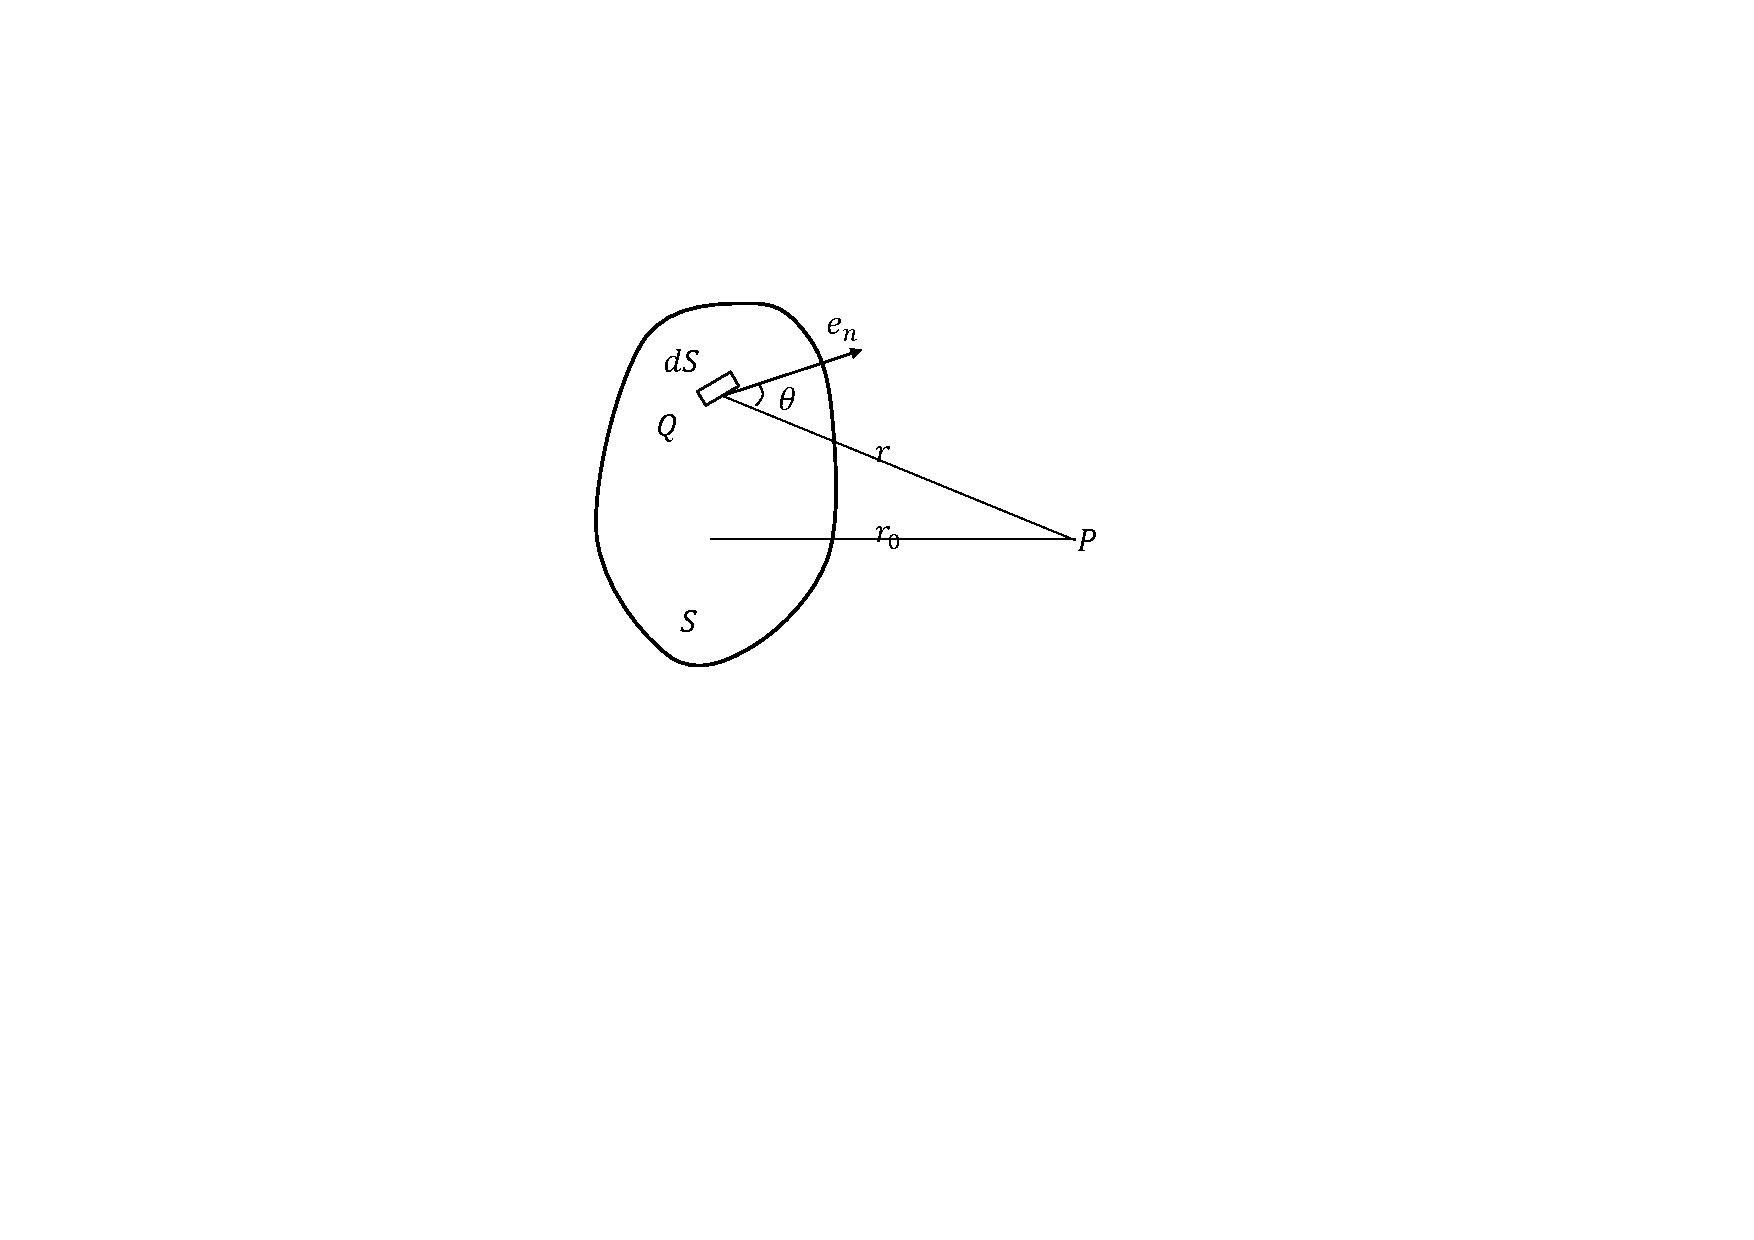
\includegraphics[width=6cm,height=4cm]{惠更斯菲涅尔原理图.pdf}}
\end{center}
\caption{惠更斯菲涅尔原理}
\end{figure*}
关键点:
\begin{itemize}
\item 球面波,振幅和r成反比
\item 从面积元发出的次波与p点的振幅反比于$\theta$所以有一个倾斜因子$K(\theta)$影响振幅
\item dS处有相同的相位
\item p点的相位为nr
\end{itemize}
这四个假设可以得到菲涅尔积分:
\[
	dE\propto\iint c\cdot \frac{dS K(\theta)}{r}\cos (\omega t-nr\frac{2\pi }{\lambda})
\]
考虑到初始振幅的分布函数$A(\theta)$对dE进行修正得到:
\[
	dE\propto\iint c\cdot \frac{dS K(\theta)A(\theta)}{r}\cos (\omega t-nr\frac{2\pi }{\lambda})
\]
\subsection{菲涅尔衍射}
\begin{figure*}[htbp]
\begin{center}
\raisebox{-0.5\height}{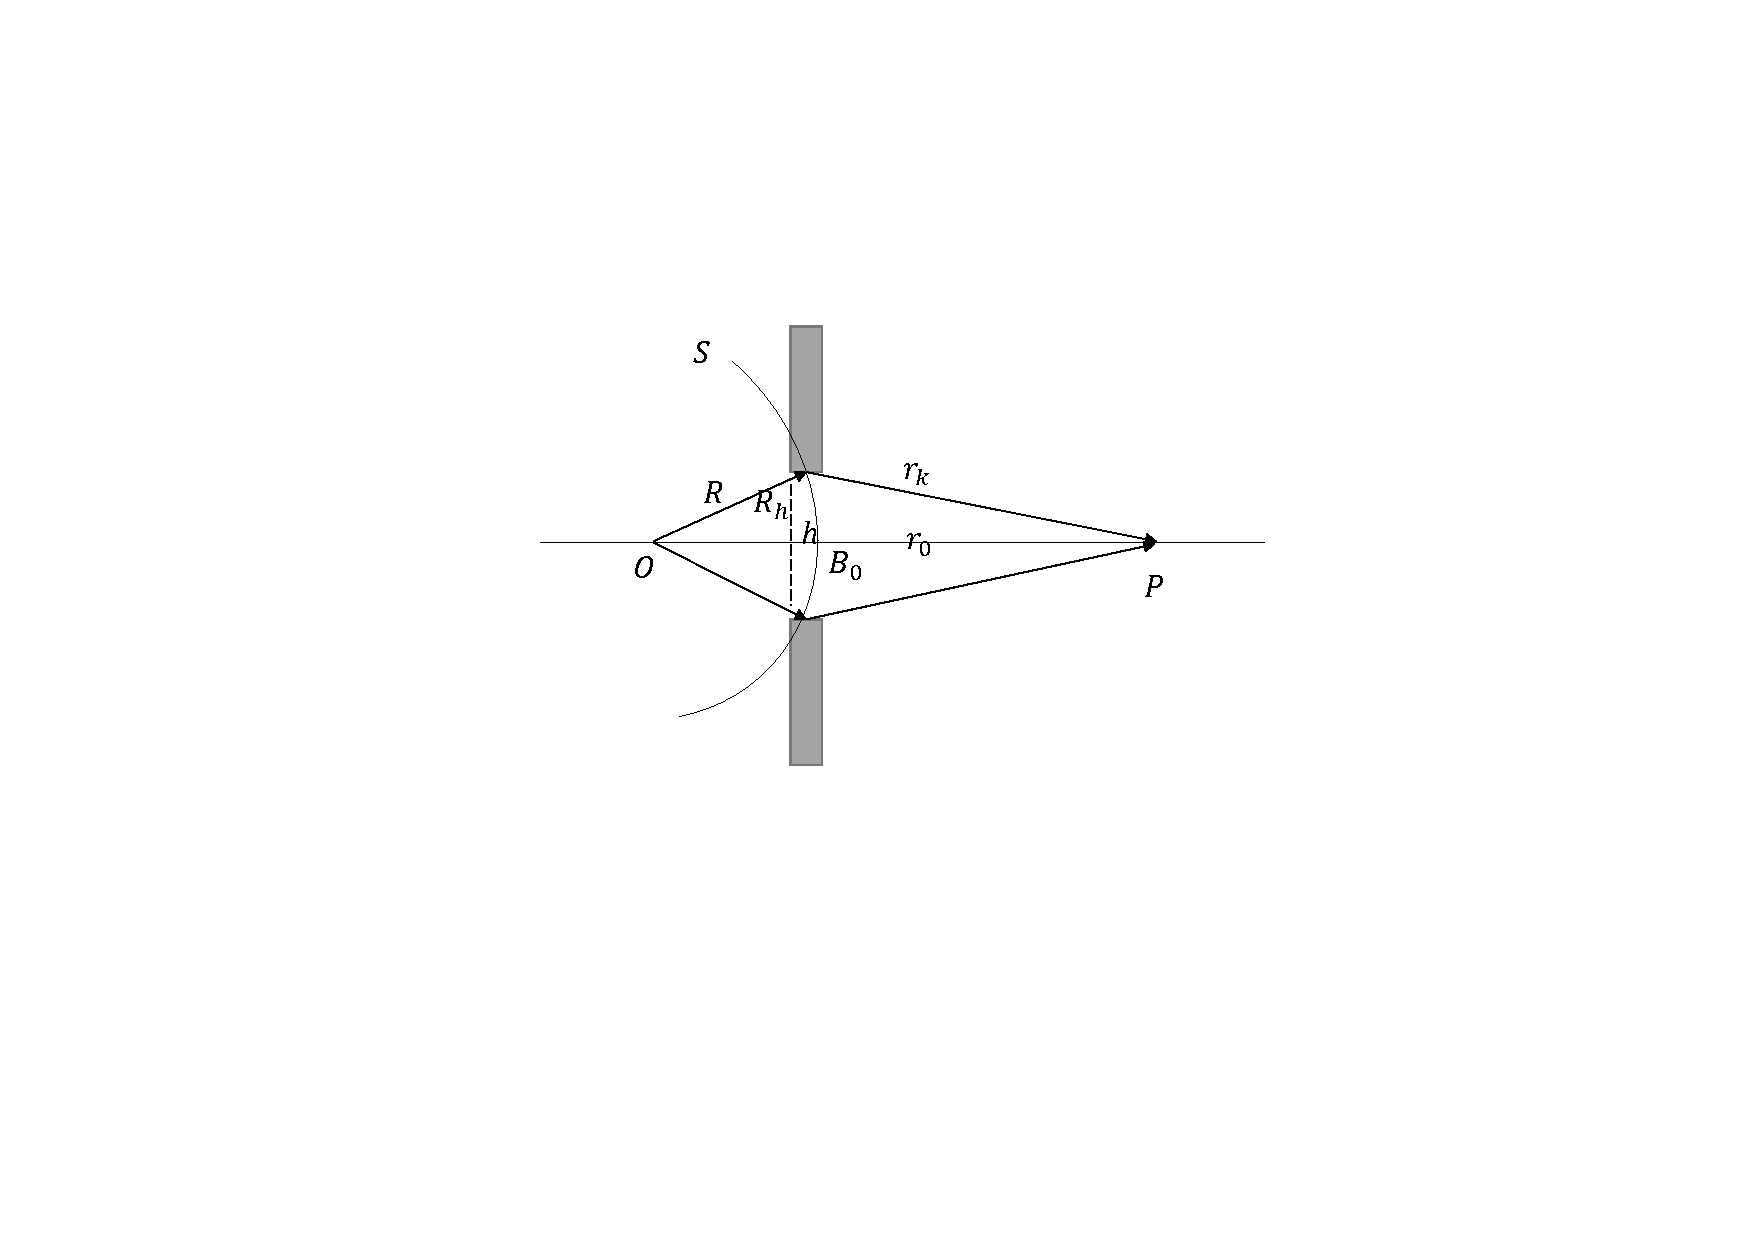
\includegraphics[width=6cm,height=4cm]{菲涅尔衍射示意图.pdf}}
\end{center}
\caption{菲涅尔衍射示意图}
\end{figure*}
我们所需要求得是$\frac{dS}{r_k}$的关系:
\begin{gather*}
S=2\pi r h=2\pi  R\cdot R(1-\cos\varphi)\\
\cos\varphi=\frac{R^2+(R+r_0)^2-r_k^2}{2R(R+r_0)}\\
dS=2\pi R^2\sin\varphi d\varphi\frac{r_k dr_k}{R(R+r_0)}\\
\frac{dS}{r_k}=\frac{2\pi R^2 dr_k}{R(R+r_0)}
\end{gather*}
当$r_k\gg \lambda$时,可以近似$dr_k=\frac{\lambda}{2}$,则此时$\frac{\Delta S }{r_k}=\frac{\pi R \lambda}{R+r_0}$与k值无关,振幅的影响因子就只剩下了$K(\theta)$的倾斜因子,因为其缓慢减小,可以得到振幅的相应关系。\\
由之前得到的菲涅尔-惠更斯原积分得到在p点的振幅叠加
\[
	A=a_1-a_2+a_3-a_4+\cdots+(-1)^{k+1}a_k
\]
由于振幅差极小,小的可以看成连续的,得到振幅公式:
\[
	A=\frac{1}{2}(a_1+(-1)^{k+1}a_{k})
\]
圆孔衍射如图7所示很相似,则此时我们是需要球的的是k的级数与$R_h,r_k,R$的关系
\begin{gather*}
R-(R-h)^{2}=r_k^2-(r+h)^2=R_h^2\\
2Rh=r_k^2-r_0^2-2r_0h\\
r_k-r_0=\frac{k\lambda}{2}\Rightarrow r_k=r_0+\frac{k\lambda}{2}\\
2Rh=r(r_0+\frac{k\lambda}{2})^2-r_0^2-2r_0h\Rightarrow 2Rh\approx r_0k\lambda -2r_0 h\Rightarrow h=\frac{kr_0 \lambda }{2(R+r_0)}
\end{gather*}
利用高阶无穷小近似的,h很小,则:
\begin{gather*}
2Rh=R_{h}^2\Rightarrow h=\frac{R_h^{2}}{2k}\\
\frac{R_h^2}{2R}=\frac{kr_0\lambda}{2(R+r_0)}\Rightarrow k=\frac{(R+r_0)R_h^2}{Rr_0\lambda }
\end{gather*}
\subsection{波带片原理}
让光程差相差是一个波长,使得振幅全部叠加没有抵消就可以得到和凸面镜相似的聚焦效果(光程差相差一个波长,相位差相差$2\pi$,不会出现抵消现象,相差半个波长,则相位差相差$\pi $会出现抵消效果
\subsection{夫琅禾费单缝衍射}
\begin{figure*}[htbp]
\begin{center}
\raisebox{-0.5\height}{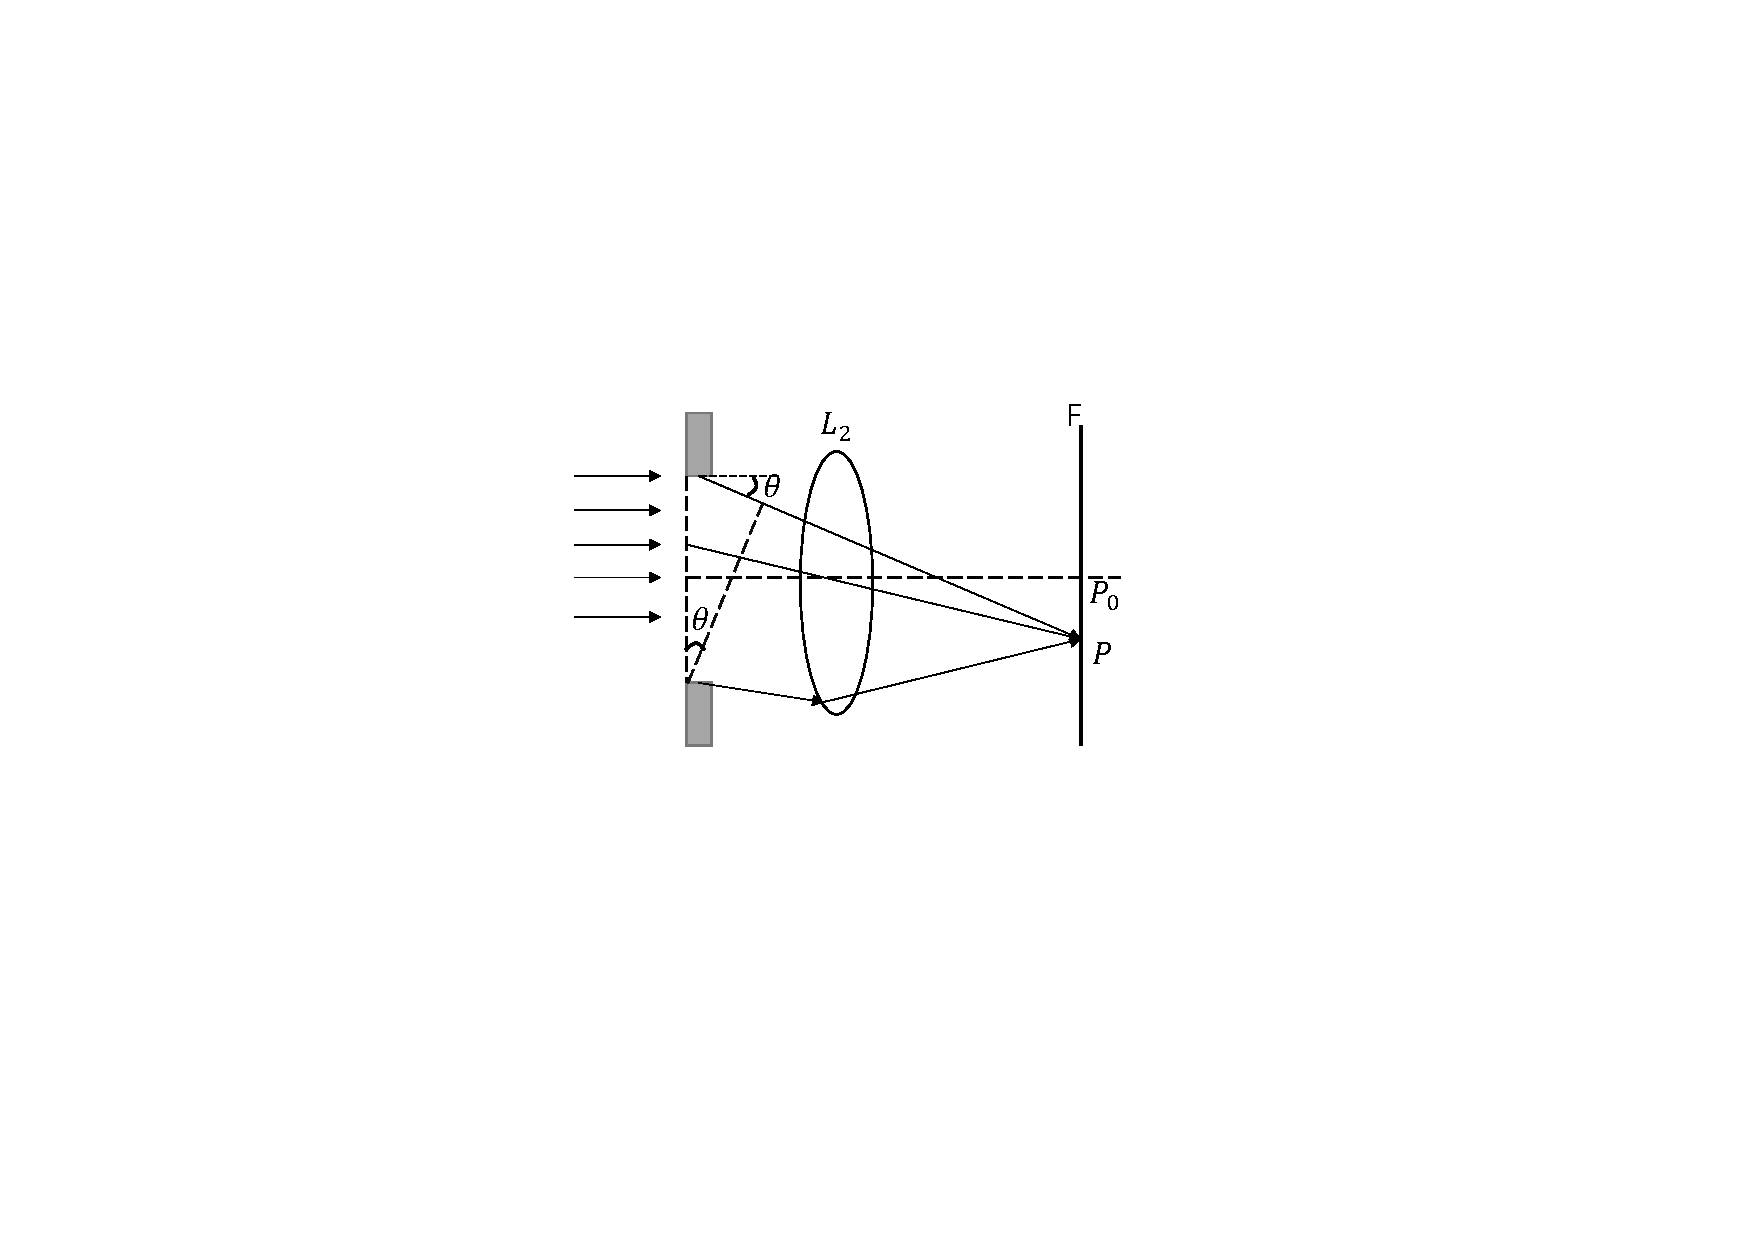
\includegraphics[width=6cm,height=4cm]{夫琅禾费.pdf}}
\end{center}
\caption{夫琅禾费衍射示意图}
\end{figure*}
夫琅禾费衍射是平行光入射,所以没有了倾斜因子的干扰此时得到对菲涅尔惠更斯积分直接进行积分可以得到;
\begin{gather*}
\int_{0}^{b}dE=\int_{0}^{b}\frac{A dx}{b}\cos (\omega t+x\sin \theta \frac{2\pi }{\lambda})\\
A=A_0\frac{\sin (\frac{\pi b}{\lambda}\sin \theta)}{\frac{\pi b}{\lambda}\sin \theta}
\end{gather*}
P点的光强可以有振幅的平方得到,然后对光强的表达式求导得到:
\begin{align*}
\begin{cases}
\sin\theta=k\frac{\lambda}{b}&\text{暗条纹}\\
\sin \theta=(k+\frac{1}{2})\frac{\lambda}{b}&\text{亮条纹}
\end{cases}
\end{align*}
\subsection{单缝衍射图样特点}
中央亮条纹的宽度:$2\frac{\lambda}{b}$\\
暗条纹的角宽度:$\frac{\lambda}{b}$\\
这里用到了$\sin \theta$近似为$\theta$\\
所以用线宽度$f\cdot \tan  \theta=f\cdot \theta$
夫琅禾费圆孔衍射
中央光斑称为艾里斑,其半角宽度$\Delta\theta=1.22\frac{\lambda}{D}$
,线宽度$\Delta l=1.22\frac{\lambda}{D}f'$
\subsection{光栅衍射-夫琅禾费多孔衍射}
\begin{figure*}[htbp]
\begin{center}
\raisebox{-0.5\height}{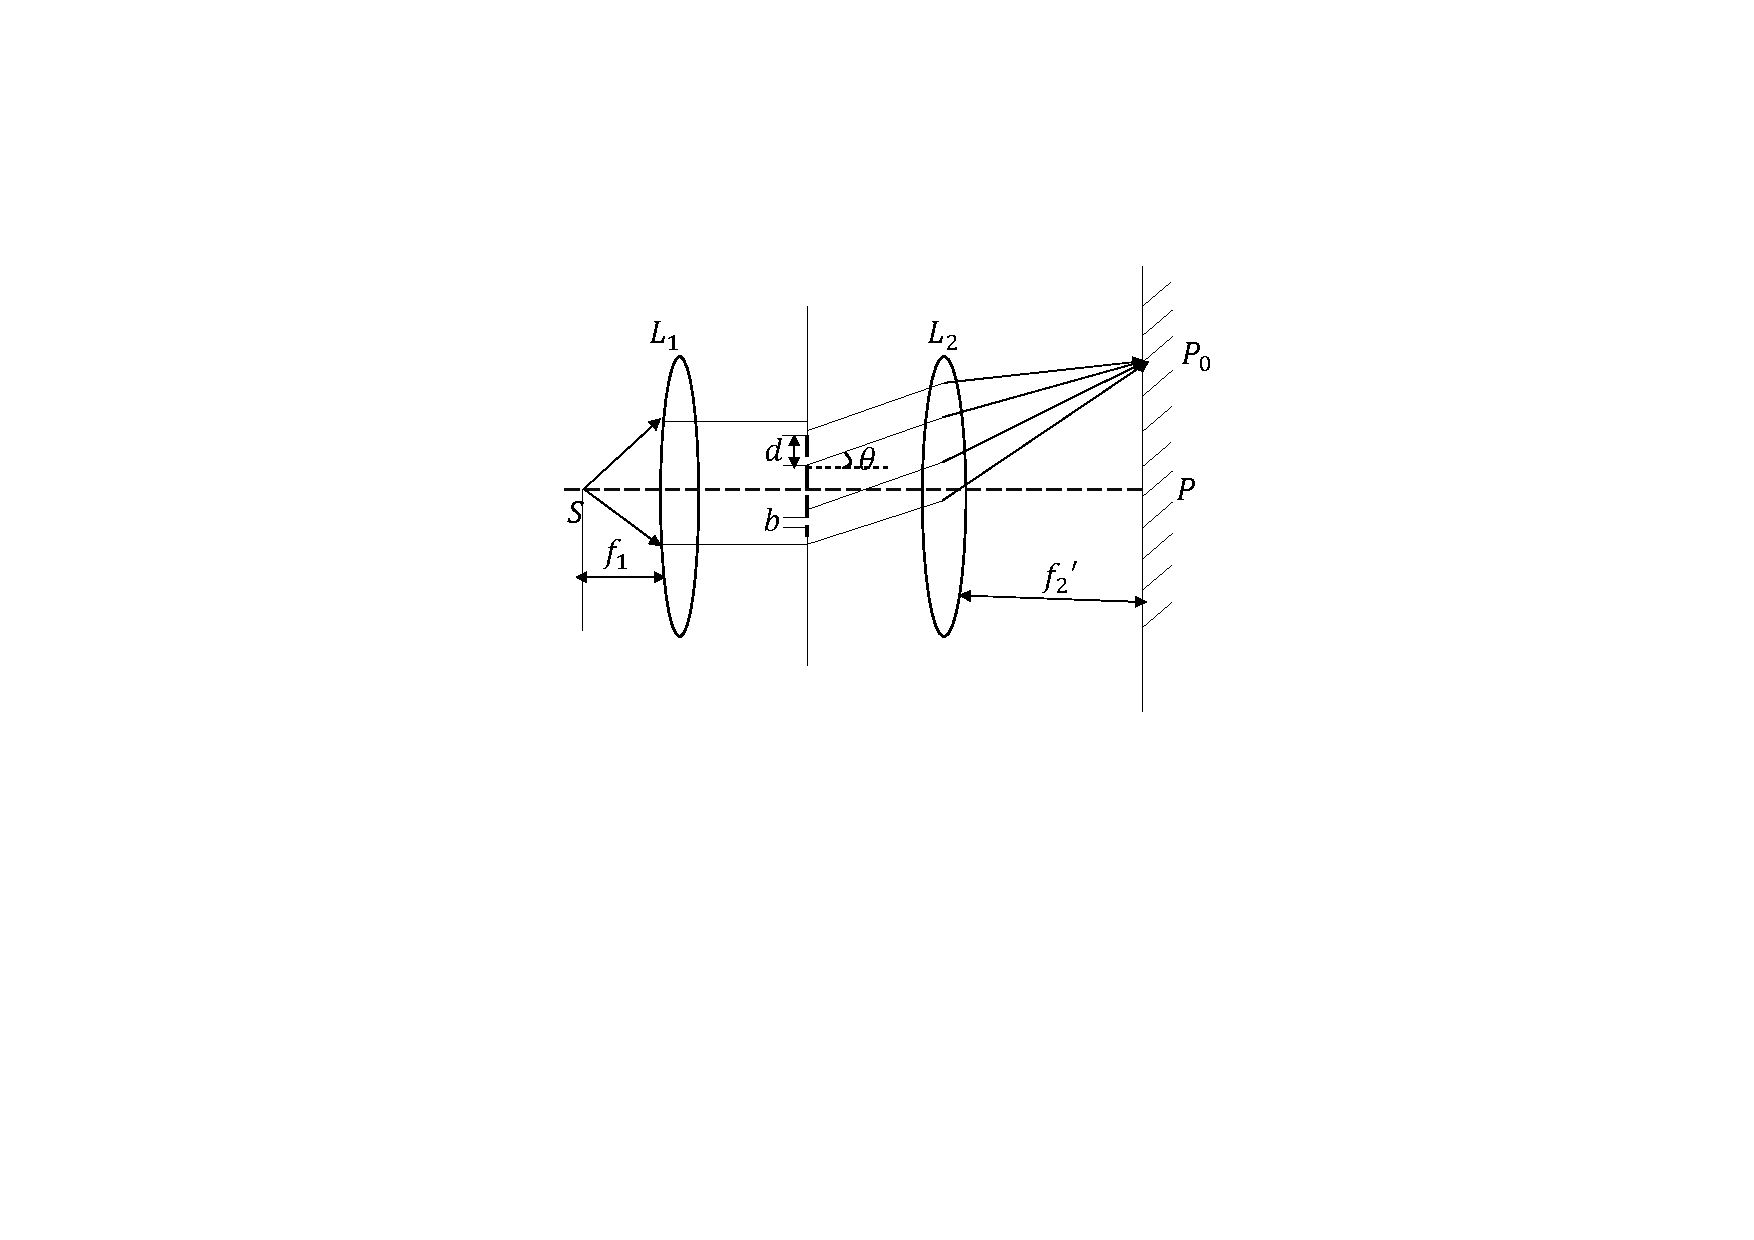
\includegraphics[width=6cm,height=4cm]{光栅.pdf}}
\end{center}
\caption{光栅衍射示意图}
\end{figure*}
现象:
\begin{enumerate}
\item 与单缝衍射相比出现一系列的主最大值和相应的亮条纹和暗条纹
\item 主最大值的宽度与缝数有关(缝数越多,宽度越窄,强度正比于$N^2$但是位置和缝数有关
\item 相邻主最大值之间有$N-1$个暗条纹和$N-2$个次最大
\end{enumerate}
半角宽度的定义:从中央明纹到第一最小值的角距离,多缝衍射因子:
\[
	\sin N(\frac{\pi d}{\lambda}\sin \theta)/\sin (\frac{\pi d}{d}\sin \theta)
\]
主最大值与主最小值:
\begin{align*}
\sin\theta=
\begin{cases}
j\frac{\lambda}{d}&(j=0,\pm 1,\pm 2\cdots)\\
j\frac{\lambda}{Nd}&(j\neq0,\pm N,\pm 2N\cdots)
\end{cases}
\end{align*}
\subsection{谱线的缺级分析}
谱线缺级就是干涉达到最大值的时候,衍射达到最小值的时候,联立两个方程,解得可以得到谱线缺级的级数
\begin{gather*}
d\sin \theta=j\lambda\\
\sin\theta=k\frac{\lambda}{b}
\end{gather*}
其中k为缺级序数,为第几次缺级,j为缺级的级数,通常算出缺级的第一个级数可以推导后面缺级的级数,
$d=4b$,则缺级的级数为$\pm 4,\pm 8,\pm 12\cdots$
类似的$d=2b$,缺级的级数:$\pm 2,\pm 4,\pm 6\cdots$
\subsection{光栅}
对于光栅光谱的分析,当复色光入射时,不同波长的光会发生叠加,波长不同的同级谱线的集合构成称为光栅光谱。第一次重叠和第二次重叠的现象时第二级和第三级\[
	j\frac{\lambda_{red}}{d}=(j+1)\frac{\lambda_{blue}}{d}
\]
光谱重叠现象:中间是白光,然后是如图所示的光谱:蓝色在里面,红光在外面,在同级谱线中,任意两一个波长的距离随着级数的增大而增大
推导过程:
\begin{gather*}
\sin \theta=j\frac{\lambda}{d}\\
\sin \theta'=j\frac{\lambda'}{d}\\
\Delta\theta=j\frac{\lambda-\lambda'}{d}
\end{gather*}
\section{偏振光}
偏振光分类:线偏振光,部分偏振光,椭圆偏振光,圆偏振光
\subsection{自然光}
自然光可以看成各个部分的线偏振光的叠加,可以将其分解到x方向和y方向,其中光强的大小:
\[
	I_{x}=I_{y}=A_{x}^{2}+A_{y}^{2}=\frac{I}{2}
\]
在整个传播过程中,若光矢量的振动只限于某一确定的平面之内,则该光为平面偏振光。其光矢量在垂直于传播方向的平面上的投影为一条方向不变的直线,故也可以称为线偏振光。\textbf{自然光通过旋转的检偏器光强不发生变化,但是变成线偏振光,而线偏振光经过旋转的偏振片,光强会发生变化},当有一个检偏器和一个偏振片时,这样我们就可以得到马吕斯定理:透过一个偏振片时有一下公式:
$I_{1}=\frac{I_0}{2}$,透过两个偏振片时:$I_2=I_1\cos^2\alpha=\frac{I_0}{2}\cos^2\alpha$,多个偏振片以此类推。\\
由菲涅尔公式可以得到:反射光是由两个振幅不等,振动方向相互垂直,非相干的线偏振光的叠加。此光为部分偏振光。偏振度P:定量的描述部分偏振光的偏振程度的物理量。
\[		
	V=\frac{I_{max}-I_{min}}{I_{max}+I_{min}}
\]
\subsection{布儒斯特角和布儒斯特定律}
如图10示意:
\begin{figure*}[htbp]
\begin{center}
\raisebox{-0.5\height}{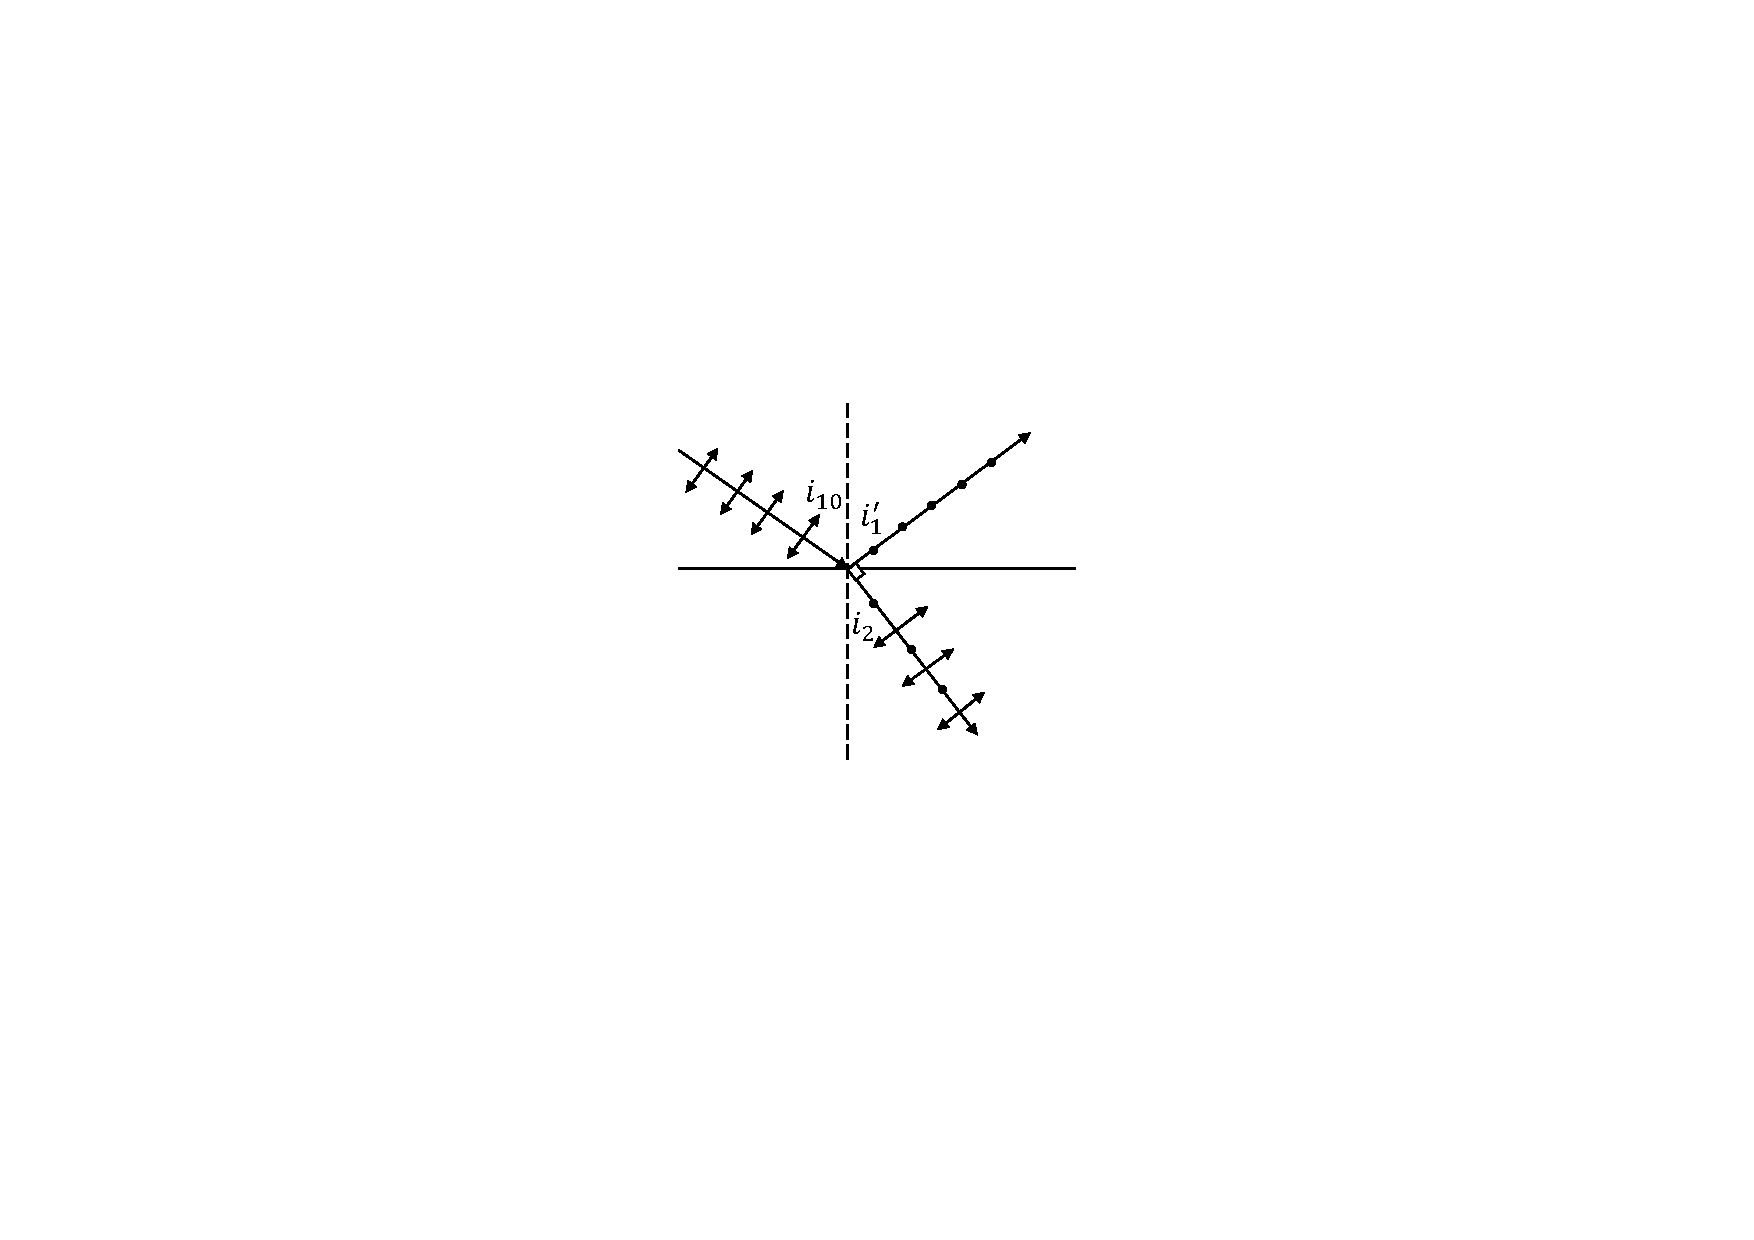
\includegraphics[width=5cm,height=4cm]{线偏振光.pdf}}
\end{center}
\caption{布儒斯特角示意图}
\end{figure*}
\begin{gather*}
\tan i=\frac{n_2}{n_1}\\
i=\arctan\frac{n_2}{n_1}
\end{gather*}
折射光为部分偏振光,且平行入射面分量强于垂直分量,当反射光线垂直于折射光线时,反射光成为线偏振光,且振动矢量垂直于 入射面
\subsection{单轴晶体的双折射现象}
在什么情况下会发生双折射:在各向同向介质遵从一般的折射定律,不会发生双折射,在各向异性介质中,会发生双折射现象。遵循折射定律的一束光成为寻常光(表示为O光),不遵循折射定律的表示为非寻常光(e光)。
如图11所示:
\begin{figure*}[htbp]
\begin{center}
\raisebox{-0.5\height}{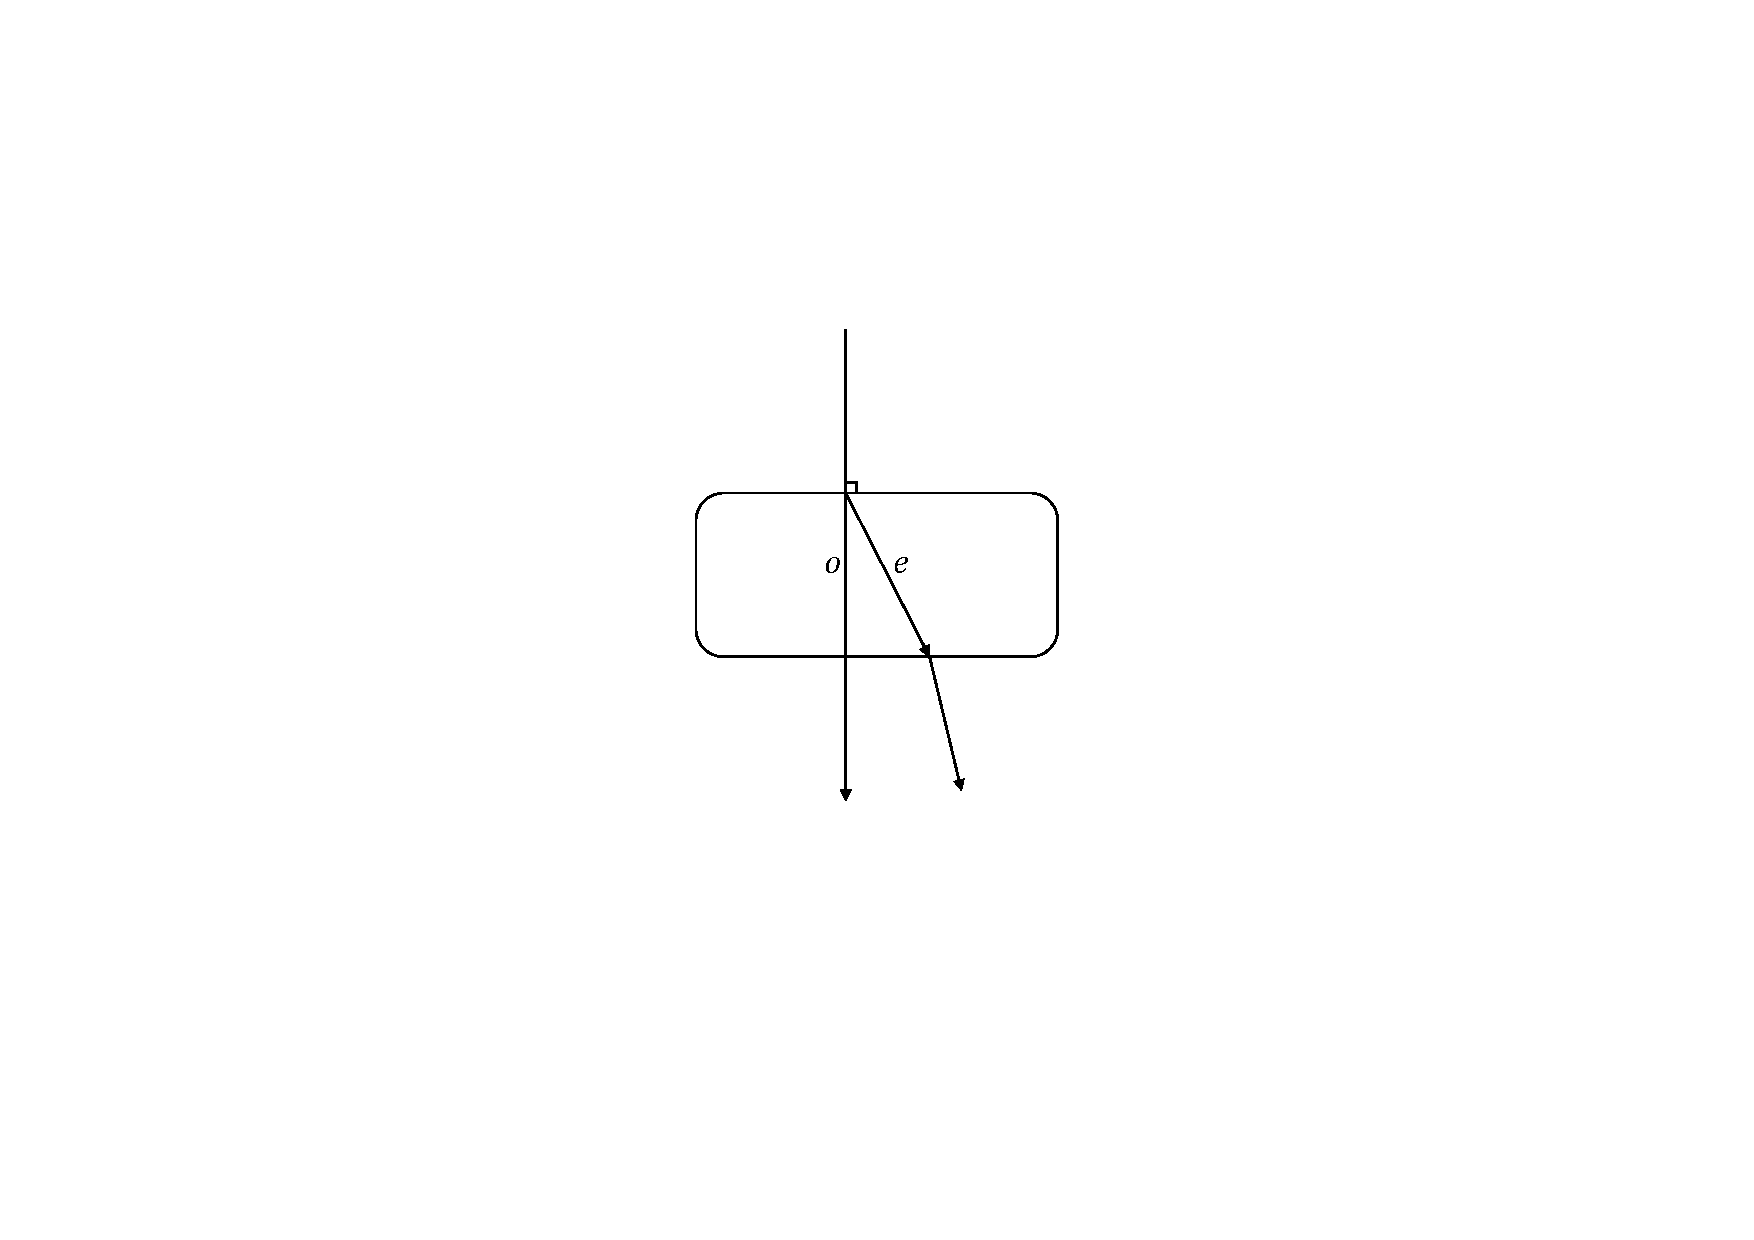
\includegraphics[width=5cm,height=6cm]{双折射.pdf}}
\end{center}
\caption{双折射示意图}
\end{figure*}
当方解石旋转时,o光不动,e光围绕o光旋转。
\subsection{光轴,主截面,主平面}
可发生双折射的晶体中不发生双折射的特殊方向成为光轴,在单轴晶体中内,由o光和光轴组成的平面称为o光的主平面,由e光和光轴组成的平面称为e光的主平面。光轴与晶体表面法线组成的平面称为晶体的主截面。如图12所示;
\begin{figure*}[htbp]
\begin{center}
\raisebox{-0.5\height}{\includegraphics[width=3cm,height=4cm]{o光.pdf}}
\qquad\qquad\qquad
\raisebox{-0.5\height}{\includegraphics[width=3cm,height=4cm]{e光.pdf}}
\end{center}
\caption{示意图}
\end{figure*}
对于自然光来说:自然光可以看成时o光和e光,且两光线的振幅相同,对于线偏振光就是不一定了。
\subsection{对于入射光是线偏振光的图像}
\begin{figure*}[htbp]
\begin{center}
\raisebox{-0.5\height}{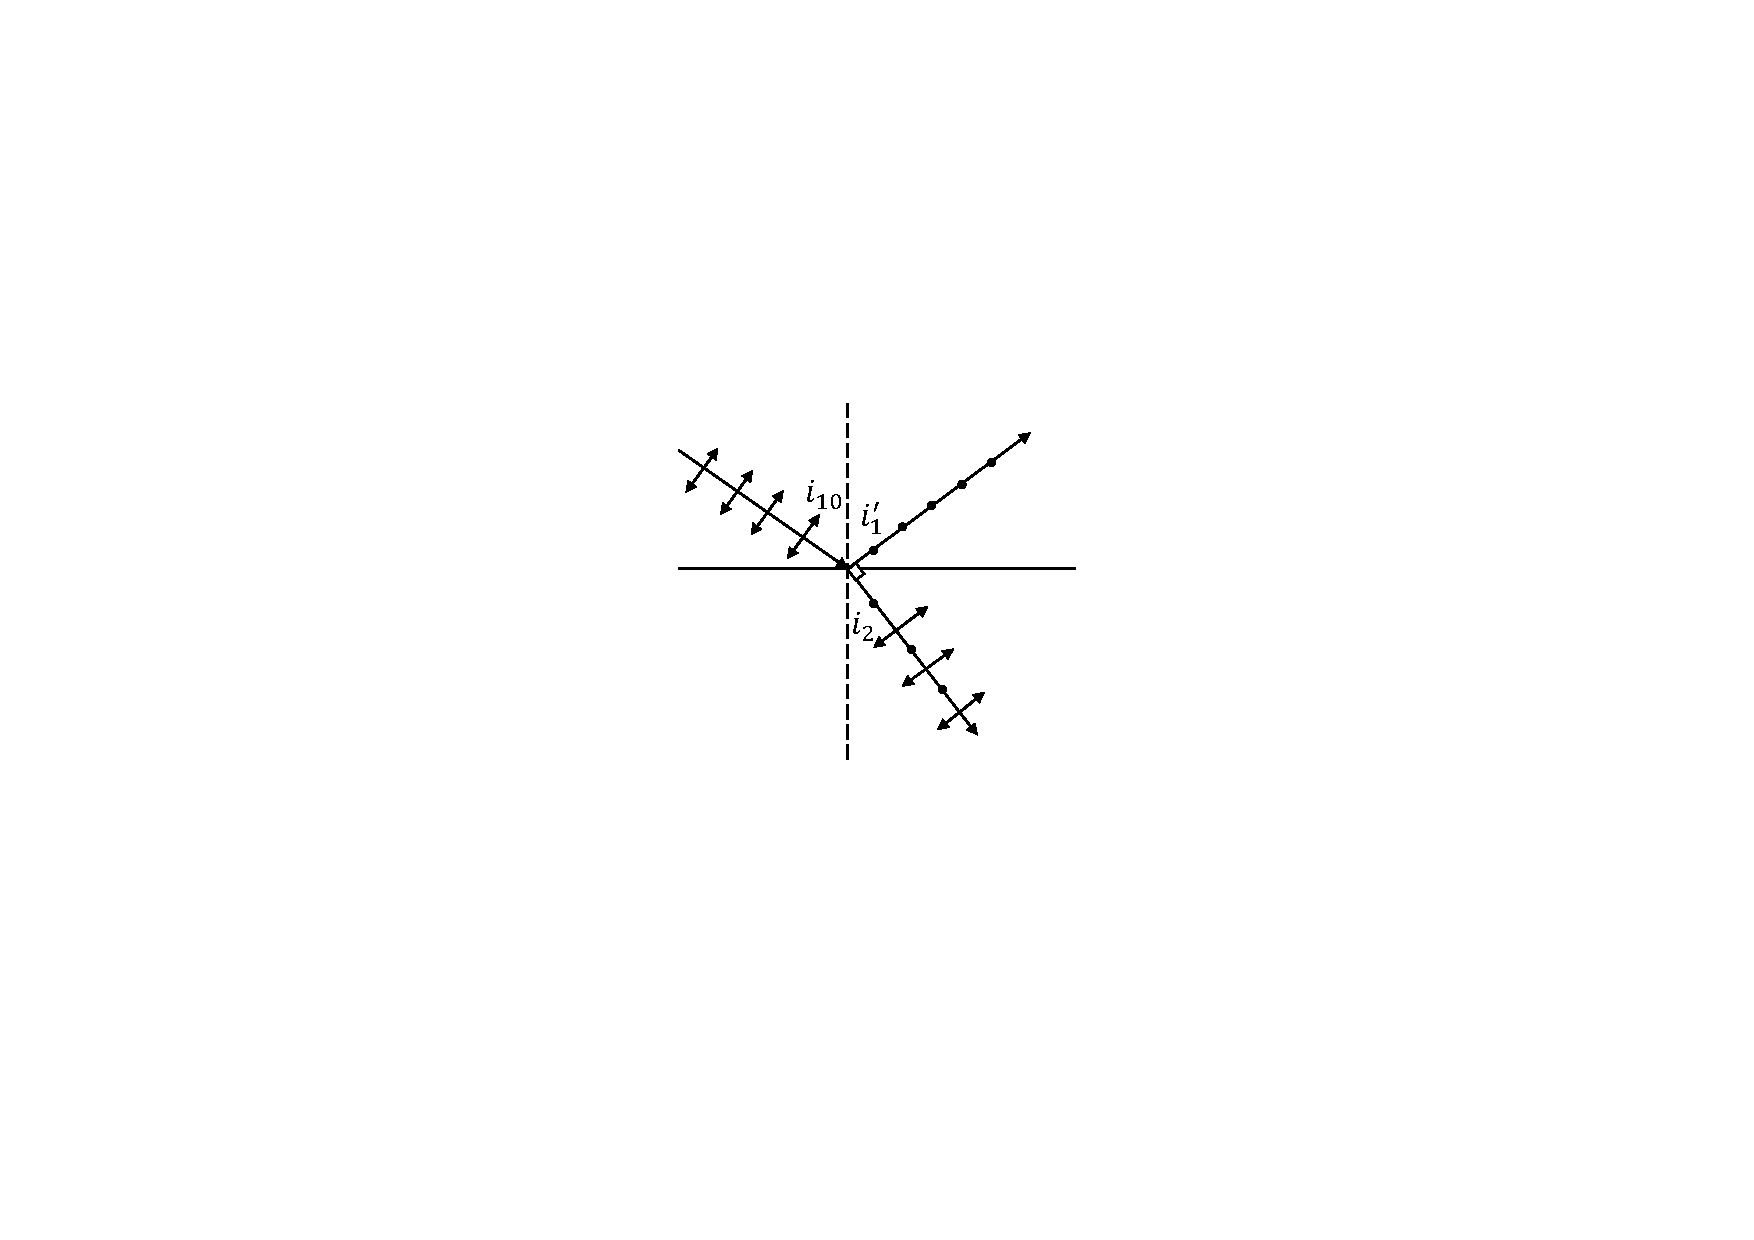
\includegraphics[width=6cm,height=5cm]{线偏振光.pdf}}
\end{center}
\caption{线偏振光示意图}
\end{figure*}
此时把入射光的震动面分解为垂直于主截面和平行于主截面,这样我们根据之前得到的:o光是垂直于主截面的,e光是平行于主截面的。
根据图13可以得到,此时的光强分析:
\begin{gather*}
A_e=A\cos \theta\\
A_o=A\sin \theta
\end{gather*}
因此光强之比:
\begin{gather*}
I_o=n_0I\sin^2 \theta\\
I_e=n_1I\cos ^2\theta\\
\frac{I_o}{I_e}=\frac{n_0}{n_1}\tan^2\theta
\end{gather*}
若将入射面扩大时,使得o光和e光的两光束重合时:
\[
	I_o+I_e=I
\]
则形成非相干叠加此时无论怎么样转换晶体,重叠部分光强不变为一常量
\subsection{光在晶体中的波面}
任意粒子的振动方向可以分为三个方向,由于振动方向的不同导致其传播速度的不同,所以形成了双折射现象
,
\end{document}